\pdfoutput=1
\documentclass[cits]{JINST}
%\let\ifpdf\relax
\newcommand{\unit}[1]{\ensuremath{\mathrm{\,#1}}}
\renewcommand{\u}[1]{\unit{#1}}
\newcommand{\um}{\textmu m}
\DeclareFontFamily{U}{euc}{}
\DeclareFontShape{U}{euc}{m}{n}{<-6>eurm5<6-8>eurm7<8->eurm10}{}%
\DeclareSymbolFont{AMSc}{U}{euc}{m}{n} % I chose AMSc because AMSa and AMSb are defined in the amsfonts-package
\DeclareMathSymbol{\umu}{\mathord}{AMSc}{"16}
\usepackage[justification=centering]{caption}
\usepackage[pdftex]{graphicx}
\usepackage{amsmath}
\usepackage{afterpage}
\usepackage{wrapfig}
\usepackage{tabularx}
\usepackage{subfigure}
\usepackage{caption}
\usepackage{tabu}
\usepackage{booktabs}
\usepackage{multicol}
\newcommand{\comment}[1]{{\fontsize{10}{10}{\par \tt\textbf {\selectfont #1}} \par}}


\graphicspath{{figs/}}


\title{Close-by showers separation within SDHCAL prototype detector using ArborPFA}

\author{R. \'Et\'e$^a$\thanks{Corresponding author.} \\%, I. Laktineh$^a$ , G. Grenier$^a$ , A. Steen$^a$ , L. Mirabito$^a$\\
\llap{$^a$} Universit\'e de Lyon, Universit\'e Lyon 1, CNRS/IN2P3, 
 IPNL, 4 Rue E.~Fermi, 69622 Villeurbanne Cedex, France\\
 
 
 E-mail: \email{rete@ipnl.in2p3.fr}
 }
 
\abstract{ After the validation of the PandoraPFA algorithm, a new reconstruction algorithm is needed in order to validate the Particle Flow Algorithm (PFA) approach. In a such designed detector, the electromagnetic calorimeters (ECAL) and hadronic calorimeters (HCAL) have a leading role in the reconstruction task. The Semi-Digital Hadron Calorimeter (SDHCAL) is a candidate prototype of hadron calorimeter for ILD since its fine granularity ($\sim$ 1cm$^2$) allows to apply the Particle Flow Algorithm. The ArborPFA algorithm has been applied to the SDHCAL detector prototype data \cite{sdhcal-paper} in order to separate close-by hadronic shower contributions. A comparison between PandoraPFA and ArborPFA has been performed. The results of this study indicate a powerful separation and a good recovered energy up to 5 cm of separation distance.}

\begin{document}

\keywords{Keywords: Particle flow; Calorimetry; ILC; SDHCAL}

\section{Introduction}
%%%%%%%%%%%%%%%%%%%%%%%%%%%%%%%%%%%%%%%%%%%
%%%%%%%%%%%%%%%%%%%%%%%%%%%%%%%%%%%%%%%%%%%

~~~~~~~After the Higgs boson discovery at LHC, a linear e$^+$ e$^-$ collider such as the ILC is foreseen in order to measure precisely its properties. An important requirement of such a machine should be a good jet energy resolution ($\Delta$E/E $\sim$3-4\%) and thus the ability to distinguish Z, W$^{\pm}$ and Higgs bosons. Since the hadronic branching fractions of these bosons is expected to be dominant, a good energy resolution and a fine transverse segmentation both must be provided by the \textit{electromagnetic calorimeter} (ECAL) and the \textit{hadronic calorimeter} (HCAL).

The calorimeters proposed by the CALICE collaboration are currently under study mainly for this purpose. A \textit{semi digital hadronic calorimeter} prototype (SDHCAL) has been constructed \cite{sdhcal-paper} and successfully tested at the CERN H2 and H6 test beam lines of the SPS (CERN) in May and August 2012 respectively. With a transverse readout segmentation of 1 cm$^2$, 48 GRPC layers of $\sim$ 2.7 cm (absorber+active medium) and a good energy resolution ($\frac{\sigma_{E}}{E}$ $\simeq$ 10 \%), this calorimeter fits perfectly the ILC needs. 

On the other hand, the Particle Flow concept has been introduced in order to achieve the ILC benchmarks \cite{ilc-tdr}. This algorithm aims to reconstruct particles using the most appropriate detector for the energy and momentum measurement. An implementation of the particle flow algorithm has been developed by M. A. Thomson \cite{pandora-pfa} and embedded in a C++ standalone framework called PandoraPFA and is, for the moment, the only mature implementation of this algorithm for linear colliders.

In this paper, we would like to present an other approach of the particle flow : the ArborPFA approach. The algorithm has been designed for high granularity calorimeters and tested on SDHCAL simulation and test beam data. First, we evaluate here the performance of the algorithm on single pion particles. Then, we present the result of a study that aims to separate two overlaid pion showers with different separation distances and different energies. For both studies, a comparison between PandoraPFA and ArborPFA is done.

\section{The Arbor particle flow algorithm}
%%%%%%%%%%%%%%%%%%%%%%%%%%%%%%%%%%%%%%%%%%%
%%%%%%%%%%%%%%%%%%%%%%%%%%%%%%%%%%%%%%%%%%%

\subsection{Principle} 
%%%%%%%%%%%%%%%%%%%%%%%%%%%%%%%%%%%%%%%%%%%

~~~~~~~The Arbor approach has been developed by H.Videau in the ALEPH experiment at LEP and adapted by M.Ruan \cite{arbor-manqi} for ILD detector design. It is based on the idea that the shower reconstruction looks like the shower structure itself : a tree topology. 

The figure \ref{ARBOR_STRUCTURE} shows the shower development after a proton interaction (left) for which we can see the multiple components of the shower : charged particles, neutral particles, electromagnetic and hadronic parts. 
In the calorimeter view, we can see the shower tree after ArborPFA reconstruction which shows also the analogy between vertexes versus calorimeter hits and particle trajectories versus connector links

With such an approach, the shower reconstruction follows a principle close to the underlying physics and can be useful for studying the shower structure. Such studies have already been done by comparing the track length of Monte-Carlo particles produced within a shower and branch lengths in reconstructed Arbor trees \cite{arbor-manqi}.
  
\begin{figure}[!ht]
  \begin{center}
    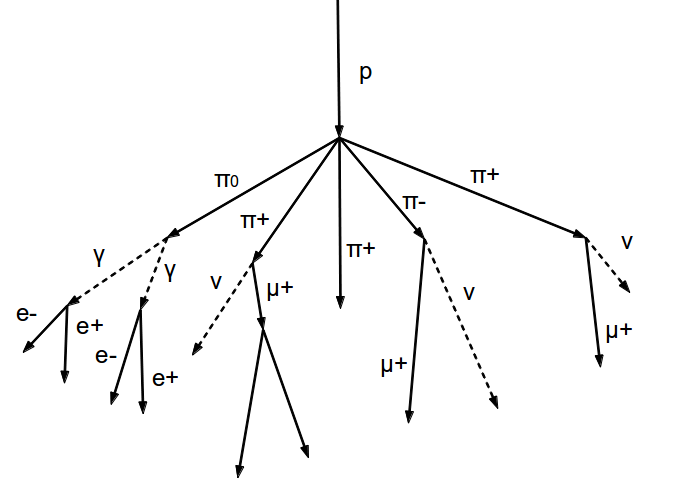
\includegraphics[width=0.45\linewidth]{ProtonDecay.png} \hfill
    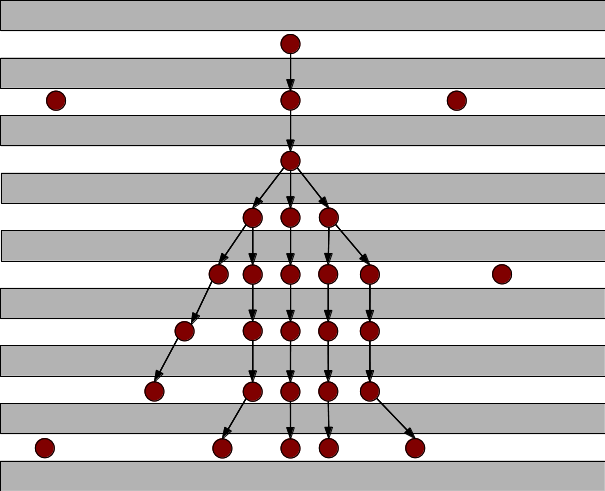
\includegraphics[width=0.45\linewidth]{ArborSchema.png}
  \end{center}
  \caption{\label{ARBOR_STRUCTURE} Left : schematic view of an induced proton shower. Right : schematic view of a reconstructed shower in a calorimeter with calorimeter hits (in red) and connectors (in black) clustered in an oriented tree topology by ArborPFA}
\end{figure}

Before describing the algorithm contents in detail, we would like to introduce some vocabulary specific to ArborPFA. We will talk about :

\paragraph*{Object} An \textit{object} is a calorimeter hit or a group of contiguous calorimeter hits within a layer that serves as vertex for the ArborPFA algorithm. This was introduced for two reasons i) provide a generalization of connections between \textit{objects} without making any assumptions of what is contained in an \textit{object}, ii) fight against the multiplicity in gaseous based calorimeters such as SDHCAL \cite{sdhcal-paper}.

\paragraph*{Flow direction} The flow direction is of two types : forward direction which is from an inward layer to a forward layer and backward direction for the opposite.

\paragraph*{Connector} A connector is a link between two \textit{objects}. It has a weight and a direction.
%Each \textit{object} keeps track of the connector lists in its backward and forward flow direction. A weight can be assigned to a connector which can be useful to sort, select or take a decision on whether to keep it or remove it.

\paragraph*{Tree} A tree is a set of \textit{objects} connected in a tree topology which means that for each object there is only one backward connector. An \textit{object} without backward connector is called a seed and an \textit{object} without forward connector is called a leaf.

\paragraph*{Cluster} A cluster is a set of trees and isolated \textit{objects} which are not connected with any other \textit{object}.

\paragraph*{Particle flow object (PFO)} A particle flow object is a set of clusters and tracks which corresponds to a reconstructed particle.


\subsection{Pre-clustering phase} 
%%%%%%%%%%%%%%%%%%%%%%%%%%%%%%%%%%%%%%%%%%%

~~~~~~~Before building trees, we need to create objects to connect with each others. Once objects are created, an additional algorithm is run in order to identify isolated objects that are not part of a shower bulb. These objects will be treated in special way in the main clustering algorithm.

%%% OBJECT CREATION %%%
\begin{wrapfigure}{r}{0.4\textwidth}
  \vspace{-20pt}
  \begin{center}
    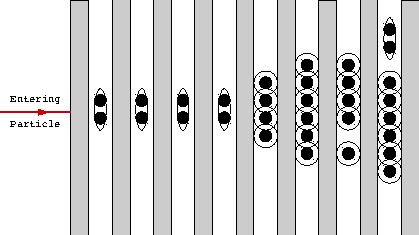
\includegraphics[width=\linewidth]{ObjectCreationAfter.pdf}
  \end{center}
  \vspace{-10pt}
  \caption{\label{ARBOR_OBJECT_CREATION} Schematic view of the object creation output. Small groups of contiguous calorimeter hits are group together (encircled).}
  \vspace{-20pt}
\end{wrapfigure}

\paragraph*{Object creation} When a minimum ionizing particle (MIP) goes through the detector, many pads can be fired in a single layer and leads to a multiplicity greater than 1. To overcome the problem, intra-layer clusters are built. For each cluster, if its number of calorimeter hits is greater than 4, the cluster is split up and each calorimeter hit becomes an object. This happens generally in the main part of a shower. In the other case, an object is created and can contains from 1 up to 4 calorimeter hits. This is the case for MIPs or isolated group of hits. 

%%% ISOLATION %%%
\paragraph*{Isolated object tagging} The second step of the pre-clustering phase consists in the identification of isolated objects that are not part of a shower bulb. For each object, we look for neighbours at a maximum distance of 18 mm in the same layer or at 5 cm in a different layer. If the number of neighbours in the same layer is greater than 3 and the total number of neighbours is greater than 1 then the object is said to be non-isolated.

\subsection{The main clustering phase - Connectors and trees}
%%%%%%%%%%%%%%%%%%%%%%%%%%%%%%%%%%%%%%%%%%%

~~~~~~~The main clustering algorithm can be decomposed in sub-algorithms i) \textit{connector seeding}, where a lot of connectors are created in order to link neighbour objects ii) \textit{connector cleaning} where some connectors are removed in order to have a tree structure and iii) \textit{tree building} where a tree is created from the connected object structure. Thanks to the modularity of the framework, it is possible to iterate on the connector seeding and cleaning algorithms. Thus, in the current implementation, a second iteration is done in order to create a connector alignment. These iteration steps are described below with more details. \\

\begin{wrapfigure}{r}{0.4\textwidth}
  \vspace{-30pt}
  \begin{center}
    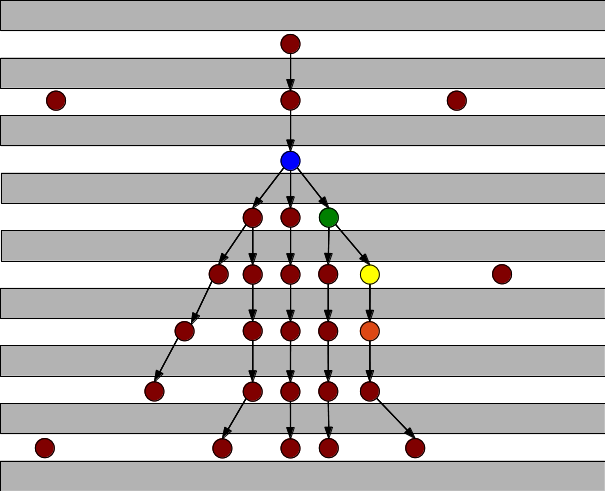
\includegraphics[width=\linewidth]{ArborConnectorDepth.png}
  \end{center}
  \vspace{-10pt}
  \caption{\label{ARBOR_CONNECTOR_DEPTH} Schematic view of the connector depth principle. Starting from the blue object, the green object has a depth of 1, the yellow a depth of 2 and the orange a depth of 3}
  \vspace{-30pt}
\end{wrapfigure}

\paragraph*{Connector seeding 1} In this sub-part, we start by creating a lot of connections in the neighbourhood of each object. For each object, we look for other objects in the next layers with a maximum distance $\Delta_{max}$ and we create a connection between them. Exception are made for isolated objects for which connections can be created only in the backward direction. In the physics point of view, this kind of objects can not lead to a forward energy deposition. Thus, a non-isolated object can be connected with an isolated object in the forward direction but not the opposite.


\paragraph*{Connector cleaning 1} Once connectors are seeded, we need to build a tree structure by keeping only one connector in the backward direction for each object. We define the reference direction of an object as :

\begin{equation}
  \vec{C_{ref}} = w_{bck} . \sum_b \vec{c_{b}} - w_{fwd} . \sum_\delta \sum_f \vec{c}_{f,\delta}
\end{equation}

where :

\begin{itemize}
  \item $w_{bck}$ is the global weight assigned to backward connectors
  \item $\vec{c_{b}}$ is the direction of a backward connector among the backward connector list
  \item $w_{fwd}$ is the global weight assigned to forward connectors
  \item $\vec{c}_{f,\delta}$ is the direction of a forward connector among the forward connector list at the depth $\delta$. The depth is a number that quantifies the number of recursive steps to reach a connector. For instance, for a given object, one of its forward connectors has a depth of 1. A forward connector of a forward connector has a depth of 2. The figure \ref{ARBOR_CONNECTOR_DEPTH} illustrates this principle. In this first cleaning, the depth is fixed to 1.
\end{itemize}

The reference direction is thus a vector that goes in the backward direction and indicate the most probable direction for a unique backward connection. Then we need to assign which backward connector should be kept for the tree building. Thus, for each of the backward connector of an object, we define the $\kappa$ order parameter as :

\begin{equation}
  \kappa~=~\Big(\frac{\theta}{2\pi}\Big)^{p_{\theta}} . ~\Big(\frac{\Delta}{\Delta_{max}}\Big)^{p_{\Delta}} 
\end{equation}

where :

\begin{itemize}
  \item $\theta$ is the angle between the backward connector and its reference direction.
  \item $\Delta$ is the distance to the backward connected object
\end{itemize}

The $\kappa$ parameter quantifies the alignment with the reference direction and is within a range [0,1]. Smaller is this parameter, higher the alignment will be. Thus, the power parameters $p_{\theta}$ and $p_{\Delta}$ are to be tuned depending on which variable we want to emphasize. 

A higher power parameter $p_{\Delta}$ will decrease the $\kappa$ parameter for the same distance between the objects and will favor the $\theta$ angle with the reference direction. In the opposite way, a higher power parameter $p_{\theta}$ will favor the distance $\Delta$ between the two objects. 

The chosen backward connector for the tree building will be the one with the smallest $\kappa$ parameter; all the others are removed from the list. The deletion of connectors is done at the end of the algorithm such that all connectors contribute to the evaluation of the reference direction.

\begin{wrapfigure}{l}{0.4\textwidth}
  \vspace{-30pt}
  \begin{center}
    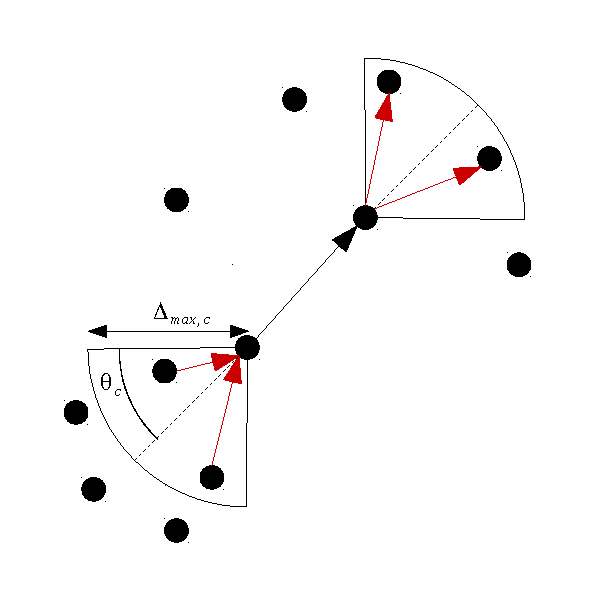
\includegraphics[width=\linewidth]{ConnectorAlignment.pdf}
  \end{center}
  \vspace{-10pt}
  \caption{\label{ARBOR_CONNECTOR_ALIGNEMENT} Schematic view of the connector alignment procedure. From an existing connection, more connections are created within a cone of angle $\theta_c$ and a distance $\Delta_{max,c}$. New connectors are in red.}
  \vspace{-30pt}
\end{wrapfigure}

\paragraph*{Connector seeding 2} This second step of connector seeding starts from the tree structure that we obtained after the first connector cleaning algorithm. The goal of this second step is to create an alignment of connectors within the shower. For each connector, more connectors are created by looking for objects in both forward and backward directions within a cone of half-angle $\theta_c$ and length $\Delta_{max,c}$. A schematic view of this step is given on figure \ref{ARBOR_CONNECTOR_ALIGNEMENT}.

\paragraph*{Connector cleaning 2} Here, we need again to clean-up the backward connector list to end up with only one connector. This last algorithm is similar to the first connector cleaning except that the cleaning is done layer per layer starting from the outer layers with a depth parameter $\delta$ greater than one. For a given connector, this accentuate the alignment with the forward ones. We end up then with a tree structure again.

~ \\
\paragraph*{Tree building} This step is straight-forward. Seed objects are identified and trees are built by taking the forward connected objects recursively. At this step, clusters are built each containing a single tree. The following association algorithms will associate some of the trees with other trees.

\subsection{Association algorithms} 

\begin{center}
  \begin{figure}[!ht]
  \subfigure[]{
    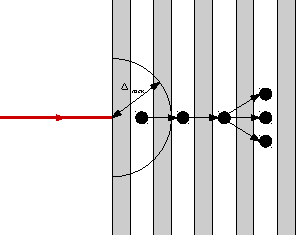
\includegraphics[width=0.5\linewidth]{TopologicalTrackAssociation.pdf}
    \label{ARBOR_TOPOLOGICAL_TRACK_ASSOCIATION}
    }
    \hfill 
  \subfigure[]{
    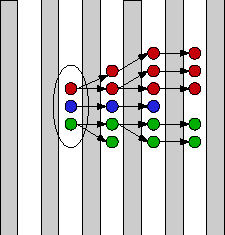
\includegraphics[width=0.38\linewidth]{NeutralTreeMerging.pdf}
    \label{ARBOR_NEUTRAL_TREE_MERGING}
    }
    \caption{(a) Topological track-to-cluster association. (b) Schematic view of a neutral hadron interaction with many seeds in the first interacting layer.}
    \label{ARBOR_ASSOCIATION_ALGORITHMS}
  \end{figure}
\end{center}

\paragraph*{Topological track association} A track to cluster association is done by using only topological information. We simply project the track entering point on the calorimeter front face. Then we look for seed objects at a maximum distance of $\Delta_{track}$. If many clusters are identified for an association, they are merged in one cluster and the association is done with the merged cluster. 

\begin{wrapfigure}{l}{0.4\textwidth}
  \vspace{-30pt}
  \begin{center}
    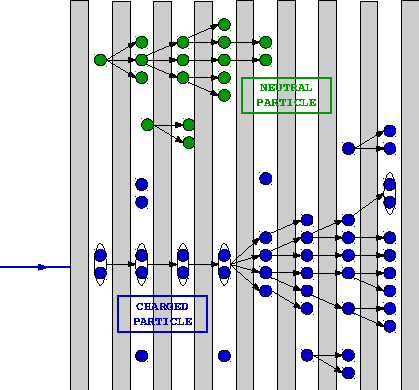
\includegraphics[width=\linewidth]{PfoCreation.pdf}
  \end{center}
  \vspace{-10pt}
  \caption{\label{ARBOR_PFO_CREATION} Schematic view of the final ArborPFA output}
  \vspace{-20pt}
\end{wrapfigure}

\paragraph*{Neutral tree merging} This algorithm is designed for neutral particle interactions for which the first interacting layer contains many seeds. The figure \ref{ARBOR_NEUTRAL_TREE_MERGING} shows a configuration where many trees have been built (with three colours) for one neutral particle interaction. We can see that the seeds in the first interacting layer should belong to the same cluster. This algorithm identifies this kind of configuration and merge the trees into one cluster.

\paragraph*{Small neutral fragment merging} At this stage, the main part of the shower of each particles has been identified. It remains only isolated objects and small tree structures that surrounds the showers. First, these small structures are identified if their size is less than $N_{cut}$ objects. Then for all showers and small structures, the centroid (barycentre) is computed and each small structure is merged in the shower that has the smallest distance between centroids.


\paragraph*{Particle flow object creation} Particle flow objects are built from the produced clusters after all the steps described above (Figure \ref{ARBOR_PFO_CREATION}). Charged PFOs are built from clusters that have an associated track, while other clusters are considered as neutral PFOs.



% %%%%%%%%% Simulation and test-beam data selection
\section{Simulation and test-beam data - Event selection}

\subsection{The SDHCAL prototype}

The SDHCAL prototype is a sampling calorimeter which geometry consists in 48 layers alternating a 20 mm steel absorber slice and a 7 mm gas resistive plate chamber (GRPC) slice. The gas gap between the two electrodes of the GRPC is 1.2 mm. 9216 pads (96 x 96) of 1cm$^2$ compose the readout of each chamber, thus the total number of channels  comes to 442368. A complete description of the calorimeter setup and its features can be found in \cite{sdhcal-paper}. 

The test beam data used in this paper have been taken at the CERN H6 beam line of the SPS in August/September 2012. The pion event selection is also done according to \cite{sdhcal-paper}. The simulation program is a standalone Geant4 application which geometry reflects the test beam geometry setup.

\paragraph*{Reconstructed energy} The reconstructed energy is computed as follows :

%\begin{equation}
  
%\end{equation}

%%%%%% Single particle study %%%%%%
\section{Single particle study}



%%%%%% Separation of close-by hadronic showers %%%%%%
\section{Separation of close-by hadronic showers}


\section{Conclusion} 


\begin{thebibliography}{6}
\renewcommand{\hepex}[1]{\href{http://www.arxiv.org/abs/#1}{\tt hep-ex/#1}}
\renewcommand{\physics}[1]{\href{http://www.arxiv.org/abs/#1}{\tt phys.int-det/#1}}
\newcommand\nim[4]{\href{http://dx.doi.org/10.1016/#4}
  {\emph{Nucl.\ Instrum.\ Meth.} {\bf #1} (#2) #3}}



\bibitem{sdhcal-paper} 
%[1] 
Calice Collaboration, \emph{First results of the CALICE SDHCAL technological prototype}, CALICE Analysis Note CAN-037,30th November 2012

\bibitem{ilc-tdr} 
%[1] 
J. Carwardine (chair) {\it et al.},  \emph{International Linear Collider Technical Design Report}. 1) Executive Summary, 2) Physics, 3) Accelerator, 4) Detectors. 12 June 2013

\bibitem{pandora-pfa}
%[2]
M. A. Thomson, \emph{Particle Flow Calorimetry and the PandoraPFA Algorithm}, Nucl.Instrum.Meth. A611:25-40, 2009


\bibitem{arbor-manqi}
%[2]
M. Ruan, \emph{Arbor, a new approach of the Particle Flow Algorithm}, Proceeding of CHEF 2013. arXiv:1403.4784v1, 2013

\newpage

\end{thebibliography}


\clearpage
\appendix

\section{Arbor algorithm parameters}
\label{ARBOR_ALGORITHM_PARAMETERS}

\begin{center}  
  \begin{table}[!ht]
    \begin{tabu} to \linewidth {| l | X | l | X |} 
          \hline
          Parameter name & Algorithm & Value & Description \\ 
          \hline \hline
          MaxClusterSize & Object Creation & 4 & The maximum intra layer cluster size to build an object with. Else the object is split in single calo hit objects \\ 
          \hline
          IntraLayerDistance & Object Creation & 11 mm & The nearest neighbour intra layer clustering maximum distance \\
          \hline
           MaxNObjectIntraLayer & Isolation Tagging & 3 & The maximum number of near objects in the same layer above which the object in non-isolated \\
          \hline
          MaxNObjectNotInLayer & Isolation Tagging & 1 & The maximum number of near objects in a different layer above which the object is non-isolated \\ \hline
          IntraLayerMaxDistance & Isolation Tagging & 18 mm & The maximum distance within a layer for intra layer objects counter \\ 
          \hline
          NotInLayerMaxDistance & Isolation Tagging & 50 mm & The maximum distance in a different layer for objects counter \\
          \hline
          MaxInitalConnectionDistance & Main Clustering & 60.5 & The distance below which an initial connection is created \\
          \hline
          AngleInitialConnection & Main Clustering & 1.0 rad & The angle of the cone below which an initial connection is created \\
          \hline
          BackwardConnectorWeight & Main Clustering & 1 & The weight of a backward connector assigned in the reference direction vector calculation. \\
          \hline
          ForwardConnectorWeight & Main Clustering & 10 & The weight of a forward connector assigned in the reference direction vector calculation. \\
          \hline   
          ThetaPowerKappaParameter & Main Clustering & 1 & The $\theta$ angle power parameter user for the $\kappa$ parameter computation \\
          \hline
    \end{tabu}    
  \end{table}
  \begin{table}[!ht]
    \begin{tabu} to \linewidth {| l | X | l | X |}
          \hline
          DeltaPowerKappaParameter & Main Clustering & 5 & The $\Delta$ distance power parameter user for the $\kappa$ parameter computation \\
          \hline
          DepthReference & Main Clustering & 2 & The forward connector depth used for the reference vector computation \\
          \hline
          MaxTrackClusterDistance & Topological Track Association & 50 mm & The distance between the track front-face projection and a seed object position above which a track-to-cluster association can be done \\
          \hline
          MaxTrackClusterNLayers & Topological Track Association & 2 & The number of layers from the calorimeter front face above which a track-to-cluster association can be done \\ 
          \hline
          SeedSeparationMerge & Neutral Tree Merging & 25 mm & The maximum distance between two seeds in the same layer above which two trees are getting merged in the same cluster \\ 
          \hline
          MaximumNObjectsMerge & Small Neutral Fragment Merging & 10 & The maximum number of objects within a tree above which it can possibly merge in a bigger cluster \\
          \hline
          LargeDistanceMerging & Small Neutral Fragment Merging & 1000 mm & The maximum closest approach distance above which a small tree can possibly merged in a bigger one \\
          \hline
          
    \end{tabu}
  \caption{The algorithm parameters of the Arbor PFA}
  \end{table}
\end{center}


\end{document}
